
%% bare_jrnl.tex
%% V1.3
%% 2007/01/11
%% by Michael Shell
%% see http://www.michaelshell.org/
%% for current contact information.
%%
%% This is a skeleton file demonstrating the use of IEEEtran.cls
%% (requires IEEEtran.cls version 1.7 or later) with an IEEE journal paper.
%%
%% Support sites:
%% http://www.michaelshell.org/tex/ieeetran/
%% http://www.ctan.org/tex-archive/macros/latex/contrib/IEEEtran/
%% and
%% http://www.ieee.org/



% *** Authors should verify (and, if needed, correct) their LaTeX system  ***
% *** with the testflow diagnostic prior to trusting their LaTeX platform ***
% *** with production work. IEEE's font choices can trigger bugs that do  ***
% *** not appear when using other class files.                            ***
% The testflow support page is at:
% http://www.michaelshell.org/tex/testflow/


%%*************************************************************************
%% Legal Notice:
%% This code is offered as-is without any warranty either expressed or
%% implied; without even the implied warranty of MERCHANTABILITY or
%% FITNESS FOR A PARTICULAR PURPOSE! 
%% User assumes all risk.
%% In no event shall IEEE or any contributor to this code be liable for
%% any damages or losses, including, but not limited to, incidental,
%% consequential, or any other damages, resulting from the use or misuse
%% of any information contained here.
%%
%% All comments are the opinions of their respective authors and are not
%% necessarily endorsed by the IEEE.
%%
%% This work is distributed under the LaTeX Project Public License (LPPL)
%% ( http://www.latex-project.org/ ) version 1.3, and may be freely used,
%% distributed and modified. A copy of the LPPL, version 1.3, is included
%% in the base LaTeX documentation of all distributions of LaTeX released
%% 2003/12/01 or later.
%% Retain all contribution notices and credits.
%% ** Modified files should be clearly indicated as such, including  **
%% ** renaming them and changing author support contact information. **
%%
%% File list of work: IEEEtran.cls, IEEEtran_HOWTO.pdf, bare_adv.tex,
%%                    bare_conf.tex, bare_jrnl.tex, bare_jrnl_compsoc.tex
%%*************************************************************************

% Note that the a4paper option is mainly intended so that authors in
% countries using A4 can easily print to A4 and see how their papers will
% look in print - the typesetting of the document will not typically be
% affected with changes in paper size (but the bottom and side margins will).
% Use the testflow package mentioned above to verify correct handling of
% both paper sizes by the user's LaTeX system.
%
% Also note that the "draftcls" or "draftclsnofoot", not "draft", option
% should be used if it is desired that the figures are to be displayed in
% draft mode.
%
\documentclass[journal]{journal}
\usepackage{algorithm, algorithmic}

%
% If IEEEtran.cls has not been installed into the LaTeX system files,
% manually specify the path to it like:
% \documentclass[journal]{../sty/IEEEtran}





% Some very useful LaTeX packages include:
% (uncomment the ones you want to load)


% *** MISC UTILITY PACKAGES ***
%
%\usepackage{ifpdf}
% Heiko Oberdiek's ifpdf.sty is very useful if you need conditional
% compilation based on whether the output is pdf or dvi.
% usage:
% \ifpdf
%   % pdf code
% \else
%   % dvi code
% \fi
% The latest version of ifpdf.sty can be obtained from:
% http://www.ctan.org/tex-archive/macros/latex/contrib/oberdiek/
% Also, note that IEEEtran.cls V1.7 and later provides a builtin
% \ifCLASSINFOpdf conditional that works the same way.
% When switching from latex to pdflatex and vice-versa, the compiler may
% have to be run twice to clear warning/error messages.






% *** CITATION PACKAGES ***
%
%\usepackage{cite}
% cite.sty was written by Donald Arseneau
% V1.6 and later of IEEEtran pre-defines the format of the cite.sty package
% \cite{} output to follow that of IEEE. Loading the cite package will
% result in citation numbers being automatically sorted and properly
% "compressed/ranged". e.g., [1], [9], [2], [7], [5], [6] without using
% cite.sty will become [1], [2], [5]--[7], [9] using cite.sty. cite.sty's
% \cite will automatically add leading space, if needed. Use cite.sty's
% noadjust option (cite.sty V3.8 and later) if you want to turn this off.
% cite.sty is already installed on most LaTeX systems. Be sure and use
% version 4.0 (2003-05-27) and later if using hyperref.sty. cite.sty does
% not currently provide for hyperlinked citations.
% The latest version can be obtained at:
% http://www.ctan.org/tex-archive/macros/latex/contrib/cite/
% The documentation is contained in the cite.sty file itself.






% *** GRAPHICS RELATED PACKAGES ***
%
\ifCLASSINFOpdf
   \usepackage[pdftex]{graphicx}
  % declare the path(s) where your graphic files are
   \graphicspath{Images}
  % and their extensions so you won't have to specify these with
  % every instance of \includegraphics
  \DeclareGraphicsExtensions{.pdf,.jpeg,.png}
\else
  % or other class option (dvipsone, dvipdf, if not using dvips). graphicx
  % will default to the driver specified in the system graphics.cfg if no
  % driver is specified.
  \usepackage[dvips]{graphicx}
  % declare the path(s) where your graphic files are
  \graphicspath{Images}
  % and their extensions so you won't have to specify these with
  % every instance of \includegraphics
  \DeclareGraphicsExtensions{.png}
\fi
% graphicx was written by David Carlisle and Sebastian Rahtz. It is
% required if you want graphics, photos, etc. graphicx.sty is already
% installed on most LaTeX systems. The latest version and documentation can
% be obtained at: 
% http://www.ctan.org/tex-archive/macros/latex/required/graphics/
% Another good source of documentation is "Using Imported Graphics in
% LaTeX2e" by Keith Reckdahl which can be found as epslatex.ps or
% epslatex.pdf at: http://www.ctan.org/tex-archive/info/
%
% latex, and pdflatex in dvi mode, support graphics in encapsulated
% postscript (.eps) format. pdflatex in pdf mode supports graphics
% in .pdf, .jpeg, .png and .mps (metapost) formats. Users should ensure
% that all non-photo figures use a vector format (.eps, .pdf, .mps) and
% not a bitmapped formats (.jpeg, .png). IEEE frowns on bitmapped formats
% which can result in "jaggedy"/blurry rendering of lines and letters as
% well as large increases in file sizes.
%
% You can find documentation about the pdfTeX application at:
% http://www.tug.org/applications/pdftex





% *** MATH PACKAGES ***
%
\usepackage[cmex10]{amsmath}
% A popular package from the American Mathematical Society that provides
% many useful and powerful commands for dealing with mathematics. If using
% it, be sure to load this package with the cmex10 option to ensure that
% only type 1 fonts will utilized at all point sizes. Without this option,
% it is possible that some math symbols, particularly those within
% footnotes, will be rendered in bitmap form which will result in a
% document that can not be IEEE Xplore compliant!
%
% Also, note that the amsmath package sets \interdisplaylinepenalty to 10000
% thus preventing page breaks from occurring within multiline equations. Use:
%\interdisplaylinepenalty=2500
% after loading amsmath to restore such page breaks as IEEEtran.cls normally
% does. amsmath.sty is already installed on most LaTeX systems. The latest
% version and documentation can be obtained at:
% http://www.ctan.org/tex-archive/macros/latex/required/amslatex/math/





% *** SPECIALIZED LIST PACKAGES ***
%
%\usepackage{algorithmic}
% algorithmic.sty was written by Peter Williams and Rogerio Brito.
% This package provides an algorithmic environment fo describing algorithms.
% You can use the algorithmic environment in-text or within a figure
% environment to provide for a floating algorithm. Do NOT use the algorithm
% floating environment provided by algorithm.sty (by the same authors) or
% algorithm2e.sty (by Christophe Fiorio) as IEEE does not use dedicated
% algorithm float types and packages that provide these will not provide
% correct IEEE style captions. The latest version and documentation of
% algorithmic.sty can be obtained at:
% http://www.ctan.org/tex-archive/macros/latex/contrib/algorithms/
% There is also a support site at:
% http://algorithms.berlios.de/index.html
% Also of interest may be the (relatively newer and more customizable)
% algorithmicx.sty package by Szasz Janos:
% http://www.ctan.org/tex-archive/macros/latex/contrib/algorithmicx/




% *** ALIGNMENT PACKAGES ***
%
%\usepackage{array}
% Frank Mittelbach's and David Carlisle's array.sty patches and improves
% the standard LaTeX2e array and tabular environments to provide better
% appearance and additional user controls. As the default LaTeX2e table
% generation code is lacking to the point of almost being broken with
% respect to the quality of the end results, all users are strongly
% advised to use an enhanced (at the very least that provided by array.sty)
% set of table tools. array.sty is already installed on most systems. The
% latest version and documentation can be obtained at:
% http://www.ctan.org/tex-archive/macros/latex/required/tools/


%\usepackage{mdwmath}
%\usepackage{mdwtab}
% Also highly recommended is Mark Wooding's extremely powerful MDW tools,
% especially mdwmath.sty and mdwtab.sty which are used to format equations
% and tables, respectively. The MDWtools set is already installed on most
% LaTeX systems. The lastest version and documentation is available at:
% http://www.ctan.org/tex-archive/macros/latex/contrib/mdwtools/


% IEEEtran contains the IEEEeqnarray family of commands that can be used to
% generate multiline equations as well as matrices, tables, etc., of high
% quality.


%\usepackage{eqparbox}
% Also of notable interest is Scott Pakin's eqparbox package for creating
% (automatically sized) equal width boxes - aka "natural width parboxes".
% Available at:
% http://www.ctan.org/tex-archive/macros/latex/contrib/eqparbox/





% *** SUBFIGURE PACKAGES ***
%\usepackage[tight,footnotesize]{subfigure}
% subfigure.sty was written by Steven Douglas Cochran. This package makes it
% easy to put subfigures in your figures. e.g., "Figure 1a and 1b". For IEEE
% work, it is a good idea to load it with the tight package option to reduce
% the amount of white space around the subfigures. subfigure.sty is already
% installed on most LaTeX systems. The latest version and documentation can
% be obtained at:
% http://www.ctan.org/tex-archive/obsolete/macros/latex/contrib/subfigure/
% subfigure.sty has been superceeded by subfig.sty.



%\usepackage[caption=false]{caption}
%\usepackage[font=footnotesize]{subfig}
% subfig.sty, also written by Steven Douglas Cochran, is the modern
% replacement for subfigure.sty. However, subfig.sty requires and
% automatically loads Axel Sommerfeldt's caption.sty which will override
% IEEEtran.cls handling of captions and this will result in nonIEEE style
% figure/table captions. To prevent this problem, be sure and preload
% caption.sty with its "caption=false" package option. This is will preserve
% IEEEtran.cls handing of captions. Version 1.3 (2005/06/28) and later 
% (recommended due to many improvements over 1.2) of subfig.sty supports
% the caption=false option directly:
%\usepackage[caption=false,font=footnotesize]{subfig}
%
% The latest version and documentation can be obtained at:
% http://www.ctan.org/tex-archive/macros/latex/contrib/subfig/
% The latest version and documentation of caption.sty can be obtained at:
% http://www.ctan.org/tex-archive/macros/latex/contrib/caption/




% *** FLOAT PACKAGES ***
%
%\usepackage{fixltx2e}
% fixltx2e, the successor to the earlier fix2col.sty, was written by
% Frank Mittelbach and David Carlisle. This package corrects a few problems
% in the LaTeX2e kernel, the most notable of which is that in current
% LaTeX2e releases, the ordering of single and double column floats is not
% guaranteed to be preserved. Thus, an unpatched LaTeX2e can allow a
% single column figure to be placed prior to an earlier double column
% figure. The latest version and documentation can be found at:
% http://www.ctan.org/tex-archive/macros/latex/base/



%\usepackage{stfloats}
% stfloats.sty was written by Sigitas Tolusis. This package gives LaTeX2e
% the ability to do double column floats at the bottom of the page as well
% as the top. (e.g., "\begin{figure*}[!b]" is not normally possible in
% LaTeX2e). It also provides a command:
%\fnbelowfloat
% to enable the placement of footnotes below bottom floats (the standard
% LaTeX2e kernel puts them above bottom floats). This is an invasive package
% which rewrites many portions of the LaTeX2e float routines. It may not work
% with other packages that modify the LaTeX2e float routines. The latest
% version and documentation can be obtained at:
% http://www.ctan.org/tex-archive/macros/latex/contrib/sttools/
% Documentation is contained in the stfloats.sty comments as well as in the
% presfull.pdf file. Do not use the stfloats baselinefloat ability as IEEE
% does not allow \baselineskip to stretch. Authors submitting work to the
% IEEE should note that IEEE rarely uses double column equations and
% that authors should try to avoid such use. Do not be tempted to use the
% cuted.sty or midfloat.sty packages (also by Sigitas Tolusis) as IEEE does
% not format its papers in such ways.


%\ifCLASSOPTIONcaptionsoff
%  \usepackage[nomarkers]{endfloat}
% \let\MYoriglatexcaption\caption
% \renewcommand{\caption}[2][\relax]{\MYoriglatexcaption[#2]{#2}}
%\fi
% endfloat.sty was written by James Darrell McCauley and Jeff Goldberg.
% This package may be useful when used in conjunction with IEEEtran.cls'
% captionsoff option. Some IEEE journals/societies require that submissions
% have lists of figures/tables at the end of the paper and that
% figures/tables without any captions are placed on a page by themselves at
% the end of the document. If needed, the draftcls IEEEtran class option or
% \CLASSINPUTbaselinestretch interface can be used to increase the line
% spacing as well. Be sure and use the nomarkers option of endfloat to
% prevent endfloat from "marking" where the figures would have been placed
% in the text. The two hack lines of code above are a slight modification of
% that suggested by in the endfloat docs (section 8.3.1) to ensure that
% the full captions always appear in the list of figures/tables - even if
% the user used the short optional argument of \caption[]{}.
% IEEE papers do not typically make use of \caption[]'s optional argument,
% so this should not be an issue. A similar trick can be used to disable
% captions of packages such as subfig.sty that lack options to turn off
% the subcaptions:
% For subfig.sty:
% \let\MYorigsubfloat\subfloat
% \renewcommand{\subfloat}[2][\relax]{\MYorigsubfloat[]{#2}}
% For subfigure.sty:
% \let\MYorigsubfigure\subfigure
% \renewcommand{\subfigure}[2][\relax]{\MYorigsubfigure[]{#2}}
% However, the above trick will not work if both optional arguments of
% the \subfloat/subfig command are used. Furthermore, there needs to be a
% description of each subfigure *somewhere* and endfloat does not add
% subfigure captions to its list of figures. Thus, the best approach is to
% avoid the use of subfigure captions (many IEEE journals avoid them anyway)
% and instead reference/explain all the subfigures within the main caption.
% The latest version of endfloat.sty and its documentation can obtained at:
% http://www.ctan.org/tex-archive/macros/latex/contrib/endfloat/
%
% The IEEEtran \ifCLASSOPTIONcaptionsoff conditional can also be used
% later in the document, say, to conditionally put the References on a 
% page by themselves.





% *** PDF, URL AND HYPERLINK PACKAGES ***
%
%\usepackage{url}
% url.sty was written by Donald Arseneau. It provides better support for
% handling and breaking URLs. url.sty is already installed on most LaTeX
% systems. The latest version can be obtained at:
% http://www.ctan.org/tex-archive/macros/latex/contrib/misc/
% Read the url.sty source comments for usage information. Basically,
% \url{my_url_here}.





% *** Do not adjust lengths that control margins, column widths, etc. ***
% *** Do not use packages that alter fonts (such as pslatex).         ***
% There should be no need to do such things with IEEEtran.cls V1.6 and later.
% (Unless specifically asked to do so by the journal or conference you plan
% to submit to, of course. )


% correct bad hyphenation here
\hyphenation{op-tical net-works semi-conduc-tor}

\pagestyle{empty}

\begin{document}
%
% paper title
% can use linebreaks \\ within to get better formatting as desired
\title{A Reservoir Computer Training Methodology to Predict the Time Evolution of Arbitrary Points on Chaotic Attractors}
%
%
% author names and IEEE memberships
% note positions of commas and nonbreaking spaces ( ~ ) LaTeX will not break
% a structure at a ~ so this keeps an author's name from being broken across
% two lines.
% use \thanks{} to gain access to the first footnote area
% a separate \thanks must be used for each paragraph as LaTeX2e's \thanks
% was not built to handle multiple paragraphs
%

\author{DJ~Passey
\thanks{DJ. Passey is with the Department
of Mathematics, University of North Carolina at Chapel Hill,
Chapel Hill, NC, 27517 USA e-mail: djpassey@unc.edu}% <-this % stops a space
\thanks{Manuscript received November, 2, 2020}}

% note the % following the last \IEEEmembership and also \thanks - 
% these prevent an unwanted space from occurring between the last author name
% and the end of the author line. i.e., if you had this:
% 
% \author{....lastname \thanks{...} \thanks{...} }
%                     ^------------^------------^----Do not want these spaces!
%
% a space would be appended to the last name and could cause every name on that
% line to be shifted left slightly. This is one of those "LaTeX things". For
% instance, "\textbf{A} \textbf{B}" will typeset as "A B" not "AB". To get
% "AB" then you have to do: "\textbf{A}\textbf{B}"
% \thanks is no different in this regard, so shield the last } of each \thanks
% that ends a line with a % and do not let a space in before the next \thanks.
% Spaces after \IEEEmembership other than the last one are OK (and needed) as
% you are supposed to have spaces between the names. For what it is worth,
% this is a minor point as most people would not even notice if the said evil
% space somehow managed to creep in.



% The paper headers
\markboth{Journal of \LaTeX\ Class Files,~Vol.~6, No.~1, January~2007}%
{Shell \MakeLowercase{\textit{et al.}}: Bare Demo of IEEEtran.cls for Journals}
% The only time the second header will appear is for the odd numbered pages
% after the title page when using the twoside option.
% 
% *** Note that you probably will NOT want to include the author's ***
% *** name in the headers of peer review papers.                   ***
% You can use \ifCLASSOPTIONpeerreview for conditional compilation here if
% you desire.




% If you want to put a publisher's ID mark on the page you can do it like
% this:
%\IEEEpubid{0000--0000/00\$00.00~\copyright~2007 IEEE}
% Remember, if you use this you must call \IEEEpubidadjcol in the second
% column for its text to clear the IEEEpubid mark.



% use for special paper notices
%\IEEEspecialpapernotice{(Invited Paper)}



\maketitle
\thispagestyle{empty}


\begin{abstract}
%\boldmath
The abstract goes here.
\end{abstract}
% IEEEtran.cls defaults to using nonbold math in the Abstract.
% This preserves the distinction between vectors and scalars. However,
% if the journal you are submitting to favors bold math in the abstract,
% then you can use LaTeX's standard command \boldmath at the very start
% of the abstract to achieve this. Many IEEE journals frown on math
% in the abstract anyway.

% Note that keywords are not normally used for peerreview papers.
\begin{IEEEkeywords}
Reservoir computers, chaos, complex systems, prediction, machine learning.
\end{IEEEkeywords}






% For peer review papers, you can put extra information on the cover
% page as needed:
% \ifCLASSOPTIONpeerreview
% \begin{center} \bfseries EDICS Category: 3-BBND \end{center}
% \fi
%
% For peerreview papers, this IEEEtran command inserts a page break and
% creates the second title. It will be ignored for other modes.
\IEEEpeerreviewmaketitle



\section{Introduction}
% The very first letter is a 2 line initial drop letter followed
% by the rest of the first word in caps.
% 
% form to use if the first word consists of a single letter:
% \IEEEPARstart{A}{demo} file is ....
% 
% form to use if you need the single drop letter followed by
% normal text (unknown if ever used by IEEE):
% \IEEEPARstart{A}{}demo file is ....
% 
% Some journals put the first two words in caps:
% \IEEEPARstart{T}{his demo} file is ....
% 
% Here we have the typical use of a "T" for an initial drop letter
% and "HIS" in caps to complete the first word.
\IEEEPARstart{D}{ue} to their ability to replicate chaotic attractors, reservoir computers have seen a surge in popularity within the field of chaotic dynamical systems \cite{Pathak2018Phys, Pathak2018Chaos, Vlachas2020}. These machine learning models were able to capture the "climate" of attractors and maintained key dynamic properties such as Lyapunov exponents \cite{Ott2018}. 

In the case of chaotic systems, reservoir computers are able to extrapolate the future trajectory of the training orbit. However, since the systems are chaotic, small differences between orbits increase exponentially with time, and all predictions eventually diverge. While the  reservoir computers in the previously cited work can predict the future evolution of the training orbit, they cannot accurately predict the trajectory of an arbitrary point on the attractor. 

Building on existing methods, we propose a training methodology that links reservoir initial conditions to learned system initial conditions and with it, successfully predict the evolution of arbitrary points on the attractor.

\subsection{Reservoir Computers: An Accessible Machine Learning Model}
 
The success of reservoir computers in reproducing chaotic attractors suggests that they are suitable for modeling, predicting and controlling complex systems. Unlike most state of the art machine learning models, reservoir computers are within reach for most scientists and engineers. Training a reservoir computer involves computing a numerical solution to an ODE and a single least squares (or Tikhanov regression) computation. It is possible to implement a simple reservoir computer in fifteen lines of code.

Modern reservoir computers are descendants of Echo State Networks and Liquid State Machines \cite{Jaeger2001, Maass2002}. Each of these models makes use of a fixed internal network as a source of non-linearity. This "reservoir" network is never trained, instead training is focused entirely on a readout mapping that translates complicated network dynamics into useful signals. Reservoirs typically consist of complex networks, but a variety of physical systems such as circuits, optical arrays and in-vitro cell cultures were shown to successfully produce the signals needed for effective reservoir computation \cite{Tanaka2019}. Famously, researchers once used a bucket of water as a reservoir, leveraging the non-linearity of the waves to project input into a higher dimensional embedding \cite{Fernando2003}. 

Currently, researchers are exploring chaining together princial component analysis, reservoir computers, neural nets,  and support vector machines for better time series classification \cite{Bianchi2020}. In addition to developing better architectures, there is work developing better reservoirs. The field of optics shows considerable promise due to low energy cost, intrinsic parallelism and speed \cite{Rafayelyan2020}.



% needed in second column of first page if using \IEEEpubid
%\IEEEpubidadjcol

\subsection{Chaotic Systems}

\subsection{Prediction of Complex Systems}

\section{Standard Reservoir Computer Training}
In the following section, we outline standard training methodology for reservoir computers.
\begin{figure}[h]
\centering
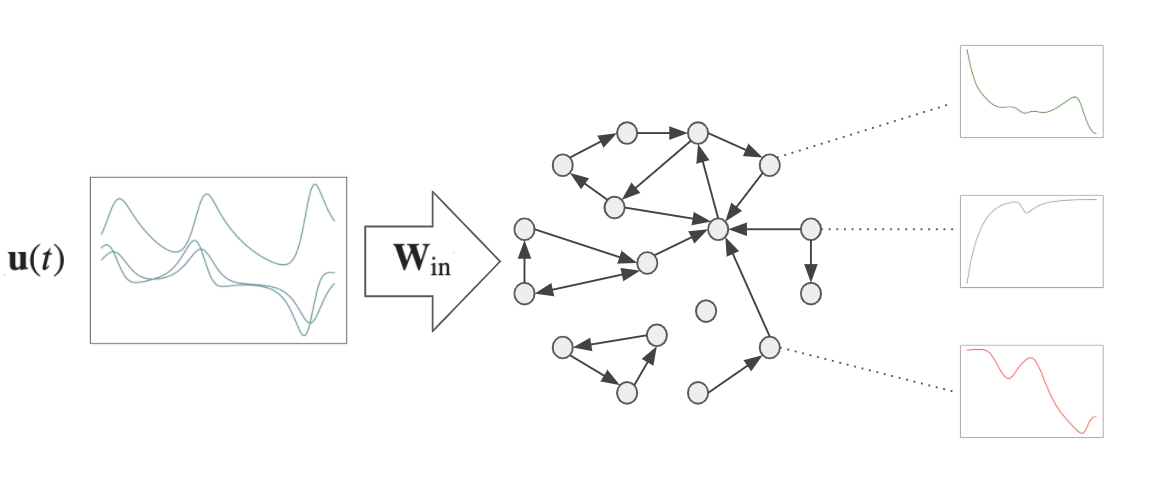
\includegraphics[scale=0.4]{Images/driven_rc_noeqs.png}
\caption{\textbf{An untrained reservoir computer driven by an input signal}}
\end{figure}


\textbf{Setup:} We create a reservoir computer as follows. 
 Let $A$ be an $n_r \times n_r$ adjacency matrix where $A_{ij}$ represents the weight of the connection from node $j$ to node $i$. 
 Let $\mathbf{r}(t)$ be an $n_r$-dimensional vector valued function of that represents the states of nodes in the network. 
 If we desire to replicate the dynamics of $\mathbf{u}(t)$ (a $n_s$ dimensional vector valued function), then we allow the reservoir nodes to evolve according to:
\begin{equation} \label{untrained}
\frac{d\mathbf{r}}{dt} = -\gamma\big[\mathbf{r}(t) + f\big(A\mathbf{r}(t) + \sigma W_\text{in} \mathbf{u}(t)\big)\big]
\end{equation}

where $\gamma > 0$ and $\sigma > 0$ are hyper parameters, $f$ is an activation function and $W_\text{in}$ is an $n_r \times n_s$ dimensional read-in matrix. In the system defined above, $A\mathbf{r}(t)$ represents recurrence, and governs how the nodes in the reservoir interact. The $W_\text{in}\mathbf{u}(t)$ term causes each reservoir node to receive a linear combination of each dimension of $\mathbf{u}(t)$.  Since $W_\text{in}$ is typically initialized randomly, each node will receive a random sum of the training data. The function $f$ should be non-linear and should be bounded to prevent the system from blowing up. Good choices for $f$ are $\tanh$ and sigmoid.

If $\mathbf{u}(t)$ for $0 \leq t \leq T$ is the training data, we proceed by discretizing the domain into $0 = t_0 <  t_1 <  ...  < t_m = T$, choosing an initial condition $\mathbf{r}_0$ (the algorithm presented here will give a thorough treatment of initial conditions) 
and using a numerical solver to solve Equation \ref{untrained} for $\mathbf{r}(t_i) \, \, i \in \{ 0, ..., m\}$.

\textbf{Learning Step: } We now seek to approximate $\mathbf{u}(t)$ with a linear combination of the reservoir states $\mathbf{r}(t)$. This is equivalent to solving for the $n_s \times n_r$ matrix $W_\text{out}$ that minimizes:
\[
\frac1m\sum_{i=0}^m \| W_\text{out} \mathbf{r}(t_i) - \mathbf{u}(t_i) \|_2
\]
This is often solved using a Tikhanov regression giving, 
\begin{equation}\label{tikhanov}
W_\text{out} = U^TR(R^TR - \alpha I)^{-1}
\end{equation}
where $\alpha$ is the regularization parameter, $R$ is a $m \times n_r$ matrix where the $i^\text{th}$ row of $R$ is equal to $\mathbf{r}(t_i)^T$ 
and $U$ is an $m \times n_s$ matrix where the $i^\text{th}$ row of $U$ is $\mathbf{u}(t_i)^T$.

\begin{figure}[h]
\centering
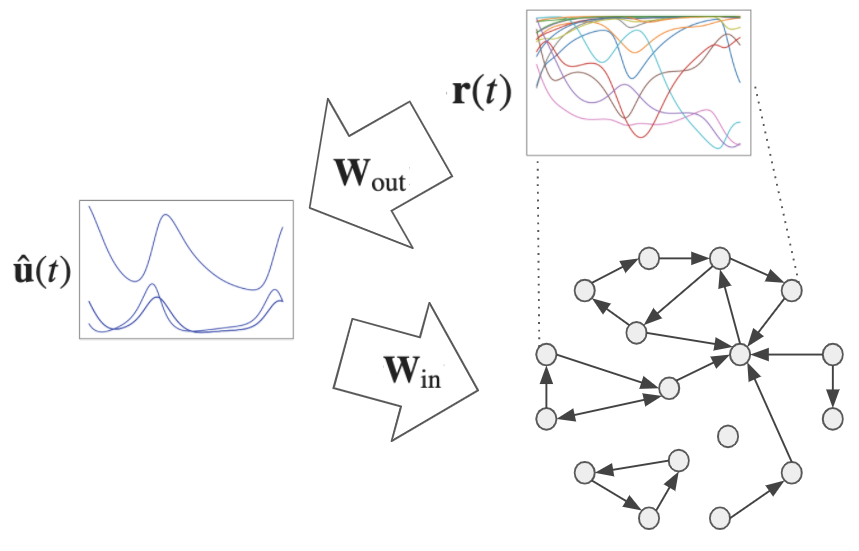
\includegraphics[scale=0.4]{Images/trained_rc_noeqs.png}
\caption{\textbf{An trained reservoir approximating the training signal without any input}}
\end{figure}

\textbf{Prediction: }
Once the readout is obtained, the reservoir computer is run as a stand-alone dynamical system to obtain a prediction. Since $\hat{\mathbf{u}}(t) = W_\text{out}\mathbf{r}(t)$ is an approximation to $\mathbf{u}(t)$ 
it is possible that for $t > T$, the approximation $\hat{\mathbf{u}}(t)$ will continue to predict $\mathbf{u}(t)$. Using the fact that $\mathbf{u}(t) \approx W_\text{out} \mathbf{r}(t)$ and substituting this into Equation \ref{untrained} produces a new equation for the evolution of node states that is independent of $\mathbf{u}(t)$:
\begin{equation}\label{trained}
\frac{d\mathbf{r}}{dt} = -\gamma\big[\mathbf{r}(t) + f\big(A\mathbf{r}(t) + \sigma W_\text{in} W_\text{out}\mathbf{r}(t)\big)\big]
\end{equation}
To predict $\mathbf{u}(t)$ for $t > T$, we need an initial condition $\mathbf{r}_0$, for the reservoir nodes. Conveniently, since $W_\text{out} \mathbf{r}(T) \approx \mathbf{u}(T)$, setting $\mathbf{r}_0 = \mathbf{r}(T)$ ensures that our reservoir node initial condition, $\mathbf{r}_0$ will map via $W_\text{out}$ to the desired system initial condition, $\mathbf{u}_0$. With  the selected $\mathbf{r}_0$ we numerically solve Equation \ref{trained} for $\mathbf{r}(t)$ when $t > T$ and apply the readout, $W_\text{out}$, to make a prediction: $\hat{\mathbf{u}}(t) = W_\text{out} \mathbf{r}(t)$.

\subsection{Problems with Existing Training Techniques}
\textbf{Problems With Random Initialization:} It is known that the prediction $\hat{\mathbf{u}}(t)$ for  $ t > T$ is not always close to $\mathbf{u}(t)$ \cite{Haluszczynski2019}. The ability of the reservoir depends on the parameters $\gamma, \sigma, A$ and $W_\text{in}$. In practice, random initialization of $A$ and $W_\text{in}$ adds some amount of variance to the predictive ability. Often, multiple reservoir computers are trained until one is found that adequately produces the desired dynamics. Statistical methods for verifying that a particular reservoir computer is "good" can be found in \cite{Haluszczynski2019}. In addition, basic hyper parameter optimization can help reduce variance in prediction ability.

Since a sparse $A$ matrix is preferable for computational efficiency, $A$ can usually be interrupted as the adjacency matrix of a network. Because most machine learning models do rely on arbitrary network structures, reservoir computing provides a link between complex network theory and learning problems. How to construct the optimal network topology is still an open question and though multiple studies on this subject exist, results are mixed \cite{Griffith2019, Pecora2019, Kawai2019}.

\textbf{Problems With Initial Conditions:} In order to produce reservoir node states from Equation \ref{untrained}, it is necessary to choose an initial condition, $\mathbf{r}_0$ from which the nodes will evolve. When picking $\mathbf{r}_0$ for the first time, there need not be any connection to $\mathbf{u}(0)$, in fact, $\mathbf{r}_0$ can be initialized randomly. When a random initialization is used, it is common to give the reservoir nodes extra time to evolve and "eliminate transients" in the node states \cite{Ott2018}. For example, researchers might use a random initial condition and solve Equation \ref{untrained} for $t \in [-T, T]$, but only use $\mathbf{r}(t)$ and $\mathbf{u}(t)$ for $t \in [0, T]$ to solve for $W_\text{out}$. 

As explained before, this method naturally lends itself to the prediction of $\mathbf{u}(t)$ for $t > T$ because $W_\text{out} \mathbf{r}(T) \approx \mathbf{u}(t)$. Thus setting the node initial condition to $\mathbf{r}(T)$ guarantees that the initial readout of the node states will be close to the desired value ($\mathbf{u}(T)$) and if the reservoir computer training was successful, $W_\text{out} \mathbf{r}(t) \approx \mathbf{u}(t)$ for $t > T$ with $\mathbf{r}(t)$ obtained by solving Equation \ref{trained}.

However, what if we want to predict the response of the learned system from an arbitrary initial condition $\mathbf{u}_0$? It is possible that if the reservoir computer was trained on appropriate data, it could extrapolate the evolution of the learned system from an unseen initial condition. The challenge here, is choosing the appropriate $\mathbf{r}_0$. Current techniques in reservoir computing for chaotic dynamical offer little insight on this subject. As such, this work will describe a methodology for choosing appropriate initial conditions and training so that reservoir computers can accurately predict the evolution of the learned system from arbitrary initial conditions.

\section{Proposed Training Methodology}

In order to predict the orbit of the learned system from a given initial condition, we need some way of linking reservoir state to the state of the system. 

While we've seen that $\mathbf{r}_0$ can be completely random and reservoir computers are still able to predict, this will not work in our case. The issue with a random initial condition is that it places reservoir nodes in an arbitrary location in the usually high dimensional reservoir space. This location in the reservoir space has no connection to the location in the system space.

\begin{figure}[h] \label{trueinitial}

\centering
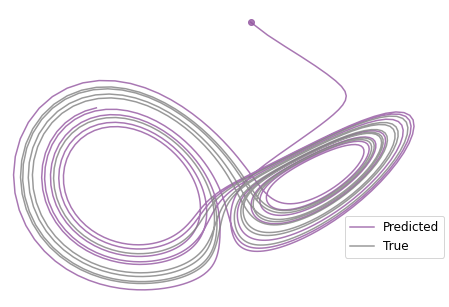
\includegraphics[scale=.25]{Images/trueinitiallorenz.png}
\caption{Standard reservoir computer prediction of the Lorenz system from an arbitrary initial condition $\mathbf{u}_0$ on the attractor. The true evolution of $\mathbf{u}_0$ is pictured in gray. The reservoir computer  prediction wanders through space for some time before settling on the attractor. Though the reservoir captures the "climate" of the Lorenz system it fails to predict the orbit of $\mathbf{u}_0$.  (For this plot, the reservoir initial state was set to $W_\text{out}^\dagger \mathbf{u}_0$.) }
\end{figure}

Since we know that $W_\text{out}$ projects the reservoir space onto the system space, it is natural to consider the pseudoinverse, $W_\text{out}^\dagger$, and apply it to $\mathbf{u}_0$ to obtain an initial condition for the reservoir. Unfortunately, this method does not work. As illustrated by Figure \ref{trueinitial}, setting the initial reservoir state in this way produces an initially transient orbit that eventually finds it's way to the attractor. It is remarkable that this orbit eventually does mimic the Lorenz system's behavior on attractor. This suggests that there is a manifold in the reservoir node space that corresponds to the Lorenz attractor, and it appears to be an attracting manifold. We can use this to our advantage.

Assuming that this attracting manifold really exists, we need to draw initial reservoir states from this manifold and also need them to be associated with the appropriate system initial condition $\mathbf{u}_0$. We can identify this manifold with the tools of nonlinear system theory.

\subsection{Reservoir Node Fixed Points} Similar to work done here: 

\textbf{https://link.springer.com/article/10.1007/s12559-019-09634-2}. 

Beginning with the untrained reservoir system,
\[
\frac{d\mathbf{r}}{dt} = -\gamma\big[\mathbf{r}(t) + f\big(A\mathbf{r}(t) + \sigma W_\text{in} \mathbf{u}(t)\big)\big]
\]
we make one simplifying assumption and let $A = \rho I$ where $I$ is the $n_r \times n_r$ identity, and $\rho > 0$ is the spectral radius. This choice removes recurrence in the reservoir and effectively decouples the system so that we can consider the evolution of reservoir nodes individually. This simplification is justified by studies showing that extremely sparse networks are more effective at learning, the benefit of recurrence is limited. With this simplification, we can study the dynamics of a single node independently with the system:
\begin{equation}\label{onenode}
\frac{dr_i}{dt} = -\gamma\big[r_i(t) + f\big(\rho r_i(t) + \sigma \mathbf{w}^T_i \mathbf{u}(t)\big)\big]
\end{equation}
Here $\mathbf{w}^T_i$ is the $i^\text{th}$ row of $W_\text{in}$. We can solve for the fixed points of this system by setting $\frac{dr_i}{dt} = 0$. This produces,
\[
-r_i = f\big(\rho r_i + \sigma \mathbf{w}^T_i \mathbf{u}(t)\big)
\]
For a given time $t_0$, let $a = \sigma \mathbf{w}^T_i\mathbf{u}(t_0)$ we have fixed points where the line $y = -r_i$ intersects the function $f(\rho r_i + a)$. Commonly used functions for $f$ include $\tanh(x), \sin(x)$ and sigmoid. Graphical analysis shows that for each of these functions, fixed points of the system will be located within $[-1, 1]$, (or more precisely, $[0, 1]$ for sigmoid).

\begin{figure}[h] \label{tanh}
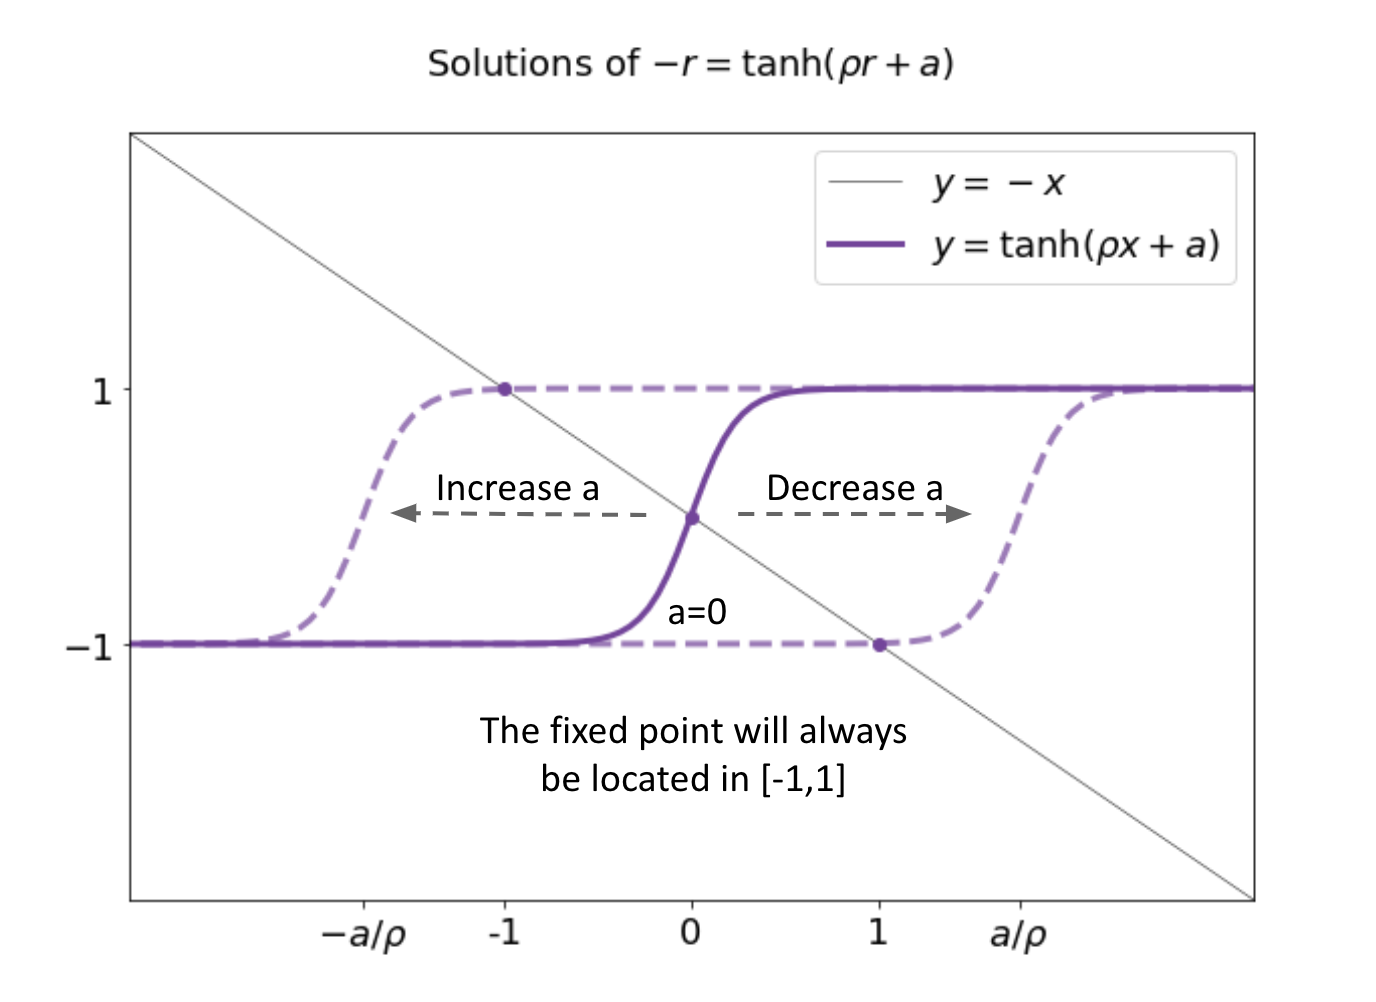
\includegraphics[scale=0.4]{Images/tanhfixed.png}
\caption{\textbf{Attracting fixed point of a reservoir node with $\tanh$ non-linearity.} In an untrained reservoir, the value of \textit{a} varies with the state of the training signal $\mathbf{u}(t)$. Therefore, the reservoir node system will have a single attracting fixed point whose location changes according to the training signal. Thus, the reservoir node will "follow" the movement of this fixed point through space as $\mathbf{u}(t)$ evolves. However, no matter the value of $\mathbf{u}(t)$, this point will always lie in [-1, 1]. (Analysis of a sigmoidal activation function is similar.)}
\end{figure}

\subsection{Stability of Reservoir Node Fixed Points}

Since the uncoupled system is one dimensional, we can compute the stability of the fixed points with,
\begin{equation}\label{stability}
\lambda = -\gamma\Big(1 + \rho f'(\rho r^\star + a) \Big)
\end{equation}
where $r^\star$ is the fixed point. If $\lambda < 0$, the fixed point is stable and attracting and it is unstable and repelling if $\lambda > 0$. 

Since $\gamma$ is positive, we know that,
 \[ 
 \lambda < 0 \,\,\text{if} \, \, 1 + \rho f'(\rho r^\star + a) > 0.
 \] 
Because $\tanh(x)$ and sigmoid have non-negative derivatives, and $\rho$ is positive, $1 + \rho f'(\rho r^\star + a) > 0$ for any $r^\star$. 

\begin{figure}[h] \label{sin}
\centering
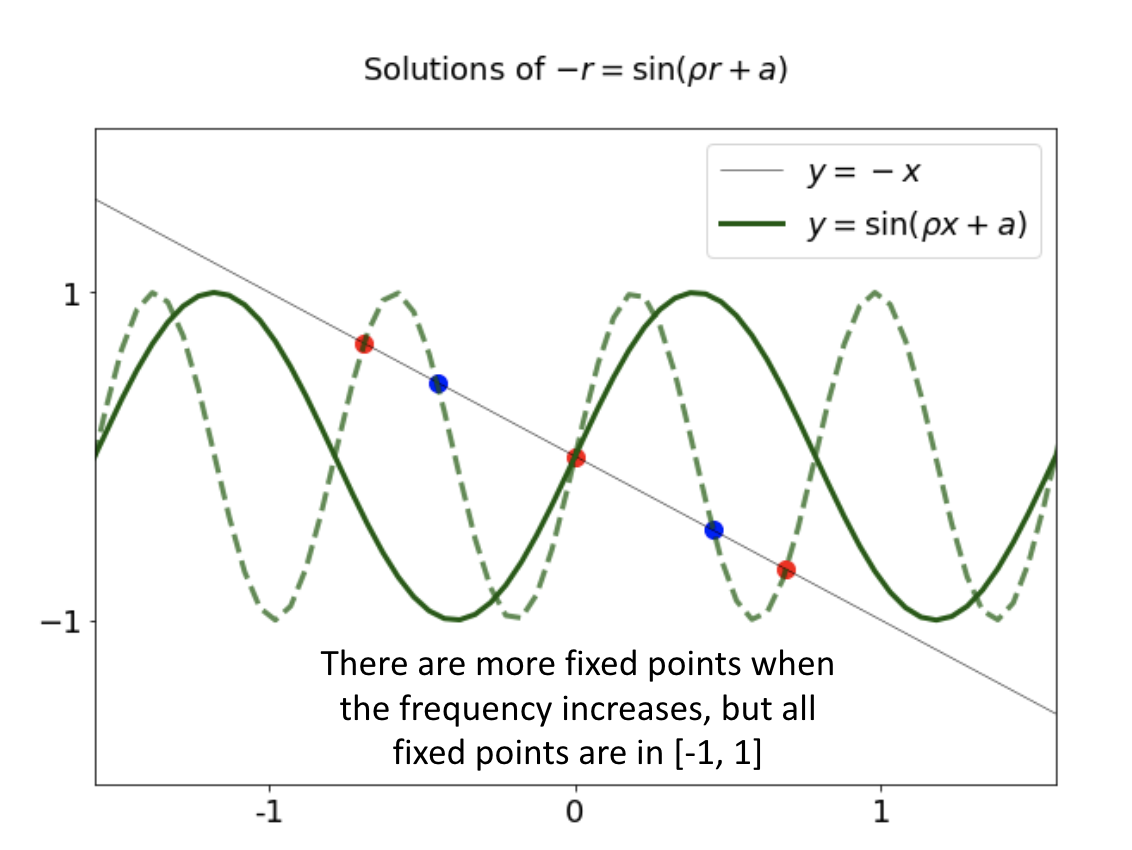
\includegraphics[scale=0.4]{Images/sinfixed.png}
\caption{\textbf{Fixed Points of a reservoir node With a $\sin$ non-linearity.} Fixed points in blue are attracting, fixed points in red are repelling. In the decoupled system, as the spectral radius increases, the number of fixed points will also increase.  Unlike $\tanh(x)$ or a sigmoidal activation function, $sin(x)$ can produce more than one fixed point which may be attracting or repelling. Combining this with the fact that $a$ changes as the training signal $\mathbf{u}(t)$ changes, creates a system of moving attracting and repelling fixed points.}
\end{figure}

Therefore, for these two activation functions, fixed points are always attracting. This is not the case when $f(x) = \sin(x)$ since it's derivative, $f'(x) = \cos(x)$ can be negative. We know that $-1 \leq \cos(x) \leq 1$, so choosing $\rho < 1$ ensures that any fixed points are attracting. However, when $\rho > 1$, the fixed points may be repelling. As pictured in figure \ref{sin}, increasing $\rho$ increases the frequency of $\sin$ which increases the number of fixed points. Because $\rho$ is larger than one, some of the fixed points are attracting (in blue) and some are repelling (in red). Combining this with the changing value of $a$ as $\mathbf{u}(t)$ changes creates potential for a complicated dynamical picture. If $\rho$ is sufficiently large, the evolving reservoir node will face a  landscape of repelling and attracting fixed points whose locations change with $\mathbf{u}(t)$. 

\subsection{A Note on Linearly Independent Node States}
Since it is the goal of a reservoir computer to project it's node states, $\mathbf{r}(t)$ onto the training signal, $\mathbf{u}(t)$, we would presume that linearly independent $r_i(t)$ would lead to better reconstruction of the training signal.

A clear way to create nearly linear \textit{dependent} $r_i(t)$ is to set $f(x) = \tanh(x)$, and use $\rho = 1$ with a large $sigma$ and positive $u(t)$ and $W_\text{in}$ with strictly positive entries. Then no matter the variation in $\mathbf{u}(t)$, if $a = \sigma \mathbf{w}_i^T \mathbf{u(t)}$ we will consistently  have $a >> 0$. Thus, the fixed point of every reservoir node will consistently remain close to -1 with very little variation in response to $\mathbf{u}(t)$. After the transient period, every reservoir node will move to -1 and stay there. This creates linearly dependent node states which would decrease the signal reconstruction accuracy. 

This un-example illustrate the importance of having fixed points in the reservoir system that move with $\mathbf{u}(t)$. The fixed points will not move as well when $a$ is large relative to $\rho$. Clearly, a $sin(x)$ activation function with a large $\rho$ will create more linearly independent node states, however, it is possible that in the mix of attracting and repelling fixed points, the nodes might lose clear correlation to the training signal.
\begin{figure}\label{sinattractor}
\centering
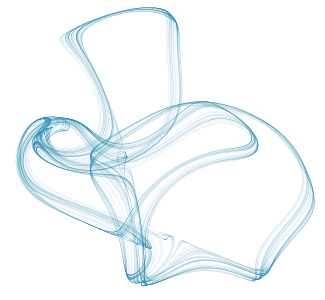
\includegraphics[scale=0.35]{Images/sinattractor.png}
\caption{\textbf{Example of reservoir nodes behaving chaotically in the absence of input with a sinusoidal activation function.} Due to the mix of attracting and repelling fixed points in a reservoir computer with a $\sin(x)$ activation function, it is not hard to create a system of reservoir nodes that behave chaotically, even without input from the training signal.}
\end{figure}
 Additionally, this mix of attracting and repelling fixed points can case the untrained system to become chaotic, even in the absence of input. The reservoir system:
 \[
\frac{d\mathbf{r}}{dt} =  -(\mathbf{r} + \sin(A\mathbf{r}))
 \] which we note is the is the untrained reservoir from Equation \ref{untrained} with $\gamma = 1, \sigma = 0$, is chaotic when 
 \[
 A = 3\pi \begin{bmatrix}
 0 & 0 & 1 \\
 1 & 0 & 0 \\
 0 & 1 & 0
 \end{bmatrix}
 \]. 
 The attractor of this system is pictured in Figure \ref{sinattractor}.
 
Since this reservoir behaves chaotically, even without input from the training  signal, it raises questions about its ability to learn. This kind of dynamic environment could make prediction more difficult, since the reservoir itself would not behave predictably. It is hard to know without further experimentation if a $sin(x)$ activation function would help or hurt a reservoir computers ability to learn.

\section{Algorithm}

\subsection{Fixed Point Initial Condition}
Based on this analysis, we will focus the remainder of the paper on $\tanh$ and sigmoidal activation functions. Bases on our fixed point analysis, we see that to eliminate transient orbits in the reservoir , the initial reservoir condition should be set to a fixed point of the reservoir system. We can compute the fixed point corresponding tp $\mathbf{u}(t) = \mathbf{u}_0$ by solving for a solution, $\mathbf{r}^\star$ to
\[
0 = -\gamma\big[\mathbf{r}(t) + f\big(A\mathbf{r}(t) + \sigma W_\text{in} \mathbf{u}_0\big)\big]
\].

Because this fixed point depends on $\mathbf{u}_0$, it associates the learned system with the internal system. Since the state of the reservoir at this point is stationary, there is no transience in the system. As $\mathbf{u}(t)$ changes with time, the location of this fixed point will move. Because we have excluded $\sin(x)$ from our analysis, the fixed point must be attracting. Thus, as it moves, the reservoir node states will follow it, synchronizing their behavior with $\mathbf{u}(t)$ immediately.
\subsection{Window Training}
\begin{figure}
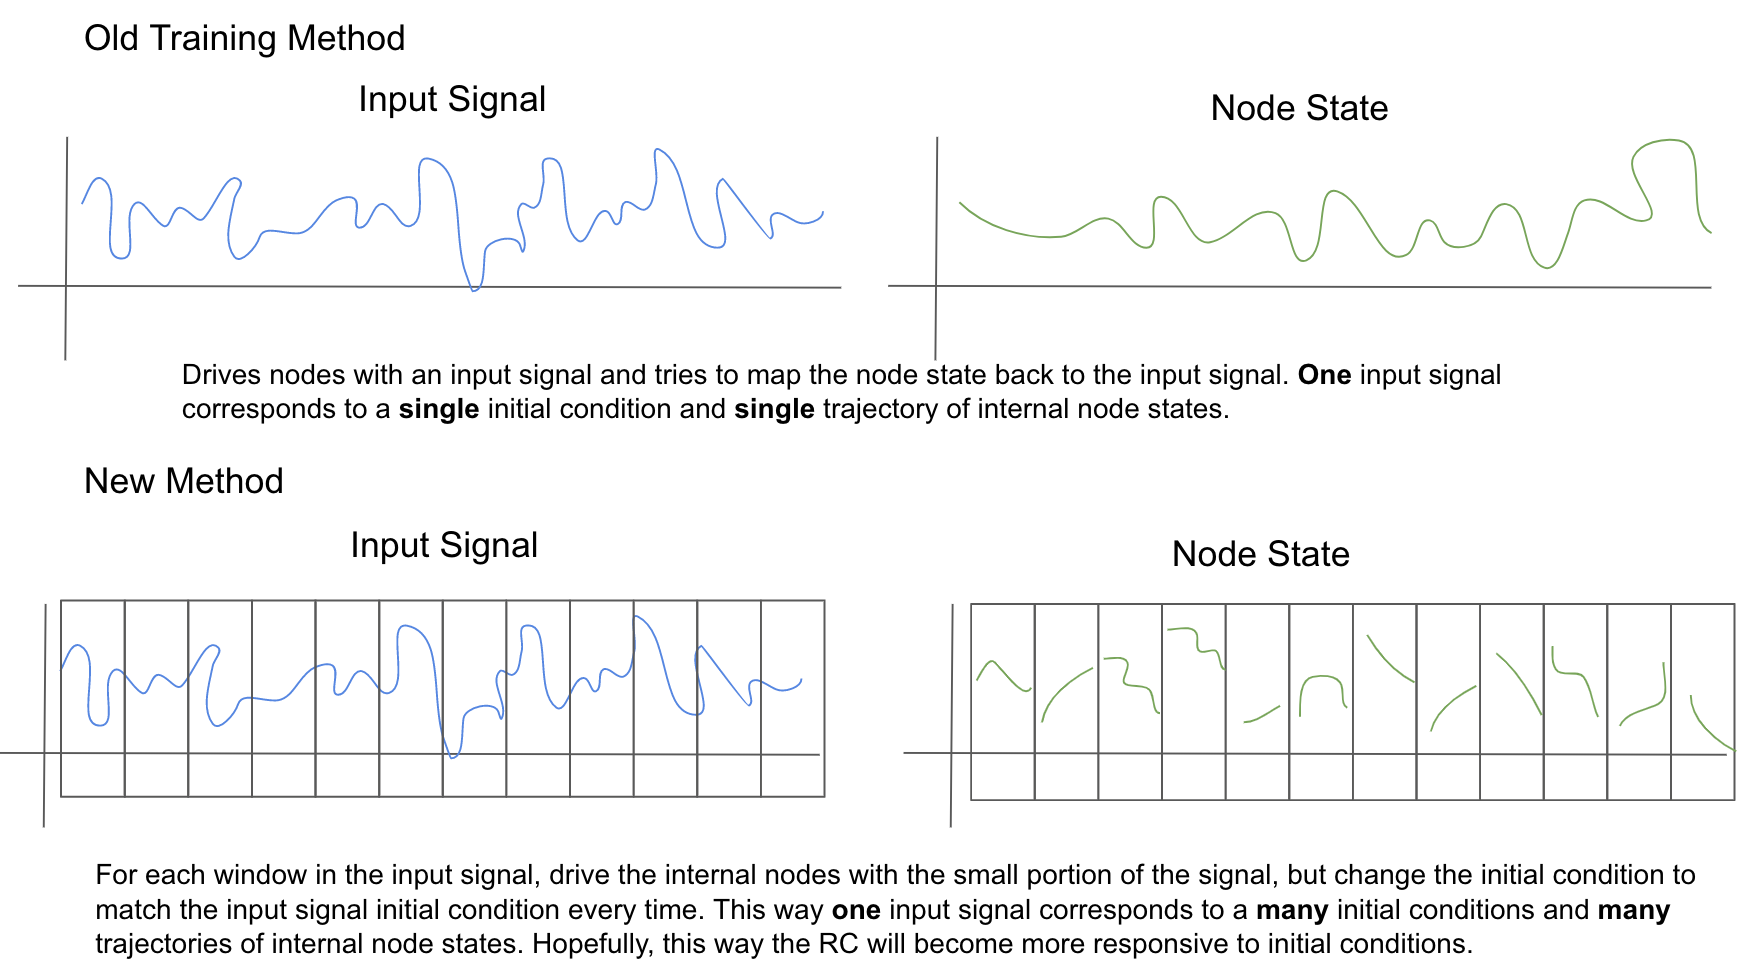
\includegraphics[scale=.3]{Images/algoexample.png}
\end{figure}

 
\begin{table*}[!t] \label{table:results}
\begin{center}
\caption{Results of testing the proposed algorithm on three chaotic systems.}
 \begin{tabular}{| c c c | c c  | c c | c c |} 
 \hline
& & System: & Rossler&  & Thomas & & Lorenz & \\ 
 \hline
& & Training Method: & Standard & Proposed & Standard & Proposed & Standard & Proposed\\
 \hline
& \multicolumn{2}{c|}{Predict Training Signal} & \textbf{59.5} & 38.6 & 20.9 & \textbf{51.2} & \textbf{6.0} & 3.97\\ 
& \multicolumn{2}{c|}{Predict Random Initial} & 0.0 & \textbf{20.7} & 0.44 & \textbf{31.9} & 0.01 & \textbf{2.21}\\
& \multicolumn{2}{c|}{System Norm} & 2.6 & \textbf{1.2} & 4.02 & \textbf{3.9} & \textbf{0.16} & 0.18\\
& \multicolumn{2}{c|}{Lyapunov Exp. Approx.} & 0.081 & 0.07 & 0.048 & 0.044 & 0.88 & 0.87\\
\hline
\end{tabular}
\end{center}
\end{table*}

Now that we have chosen a natural initial condition, we turn our focus to training the reservoir computer to learn the correspondence between learned system initial conditions and reservoir initial conditions. We do this, by exposing the reservoir computer to many initial conditions instead of just one. This is accomplished by breaking the training signal into overlapping windows and resetting the initial condition for each window.

An innovation from \cite{RNNCompare}, to break up Tikanov regression computation into batches simplifies this process:

Typically, when training a reservoir, we take an initial condition $\mathbf{u}_0$, and, using an ODE solver, generate an array $(m \times n_d)$ of samples, $U$ from the training system.
Next, we set the reservoir initial condition with $\mathbf{r}_0$ and use and ODE solver to obtain $R$, the $(m \times n_r)$ array of reservoir node states.

The training step invloves solving $||W_\text{out} R - U||_2$ for minimizer $W_\text{out}$. Tikanov regression with regularization parameter  $\alpha$ gives the solution
\[
W_\text{out} = (R^TR - \alpha I)^{-1} R^T U
\]

When $n$ is large the cost of storing $R$ in memory can be prohibitive. This problem is addressed by computing $R^TR$ and $R^TU$ in batches. We write
\[
R = [
R_1 \, \,
R_2 \, \,
R_3 \, \,
\cdots  \, \,
R_k
]^T
\]
where each $Ri$ is an $(m_i \times n_r)$ array and $\sum_i^k m_i = m$.

Then 
\[
R^TR = \sum_i^k R_i^T R_i
\]
If we break up $U$ into 
\[
U = 
[ U_1 \, \, U_2 \, \,  \cdots \, \, U_k ] ^T
\]
where each $U_i$ has dimension $(m_i \times n_d)$ we can compute $R^TU = \sum_i^k R_i^T U_i$. This allows us to compute $W_\text{out}$ in batches. If the resulting matrices, $R^TR$ and $R^TU$ are saved, $W_\text{out}$ can be updated with additional data.

When solving for $W_\text{out}$, we point out that there is no requirement that $R_i$ corresponds with $R_j$ when $j \neq i$. That is, whereas before, we assumed that $R$ was a continuous stream of node states, and $W_\text{out}$ projects $R$ onto $U$, in actuality $W_\text{out}$ attempts to send the rows of $R$ to the associated rows in $U$. Therefore, the matrix $U$ may contain orbits from multiple different initial conditions as long as the corresponding rows of $R$ are the response of the reservoir computer to those orbits and their corresponding initial conditions.

Therefore we can break up the training signal into overlapping time windows and drive the reservoir computer with each window separately. For each window, we reset the reservoir internal initial condition to correspond with the first input condition of the particular time window.  After this we can map the driven internal states back on to the concatenation of time windows. This allows us to train a reservoir computer to replicate an orbit starting from multiple places along the orbit. The number and size of time windows is a hyper parameter that can be tuned.

\section{Results}
\begin{figure}[h]
\centering
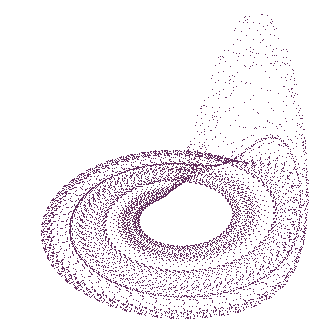
\includegraphics[scale=0.2]{Images/rosslerattractor.png}
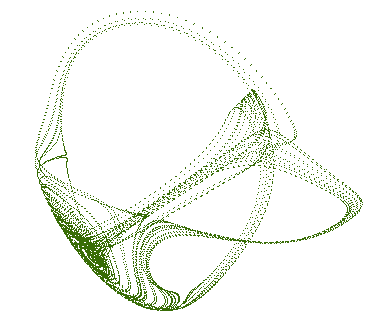
\includegraphics[scale=0.2]{Images/thomasattractor.png}
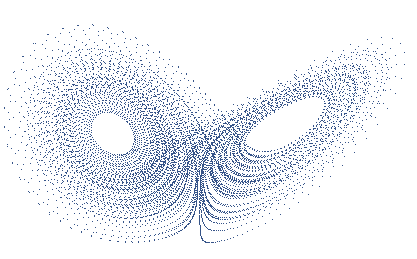
\includegraphics[scale=0.2]{Images/lorenzattractor.png}
\caption{\textbf{Chaotic systems used to test reservoir prediction from random initial points on the attractor.} In order from left to right, the Rossler attractor, Thomas' cyclically symmetric attractor, the Lorenz attractor.}
\end{figure}

To test the algorithm outlined above, 3 chaotic systems were selected: The Lorenz system, the Rossler system and Thomas' cyclically symmetric system \cite{Thomas, Lorenz, Rossler}. For each system, hyper parameters were optimized for the \textit{standard training algorithm} via a random search. These same hyper parameters were used to test the proposed new algorithm. 

For 200 different random reservoir computers, the following metrics were tested. First, the length of time that the reservoir computer could predict the training orbit with absolute error less that 0.2. Second, a random initial condition on the attractor was selected and the length of time that the reservoir computer could predict the evolution of this random initial condition with absolute error less than 0.2 was recorded. 

\textbf{Solution Error} We measured how well the orbit predicted by the reservoir solved the given system equations. Our approach here was to interpret a reservoir computer prediction as a continuous function $\hat{\mathbf{u}}(t)$. Since the reservoir computer is trying to learn a system of the form $\mathbf{u}'= F(\mathbf{u}, t)$, a successful prediction, $\hat{\mathbf{u}}(t)$, should be a solution the the equation above. That is,
\[
\hat{\mathbf{u}}' = F(\hat{\mathbf{u}}, t)
\]
if $\hat{\mathbf{u}}(t)$ is a perfect prediction. We can therefore measure the degree that $\hat{\mathbf{u}}(t)$ is not a solution with the expression,
\[
\| F(\hat{\mathbf{u}}(t), t) - \hat{\mathbf{u}}'(t) \|
\]

Because computation of $\hat{\mathbf{u}}(t)$ in practice results in the discrete values, $\hat{\mathbf{u}}(t_i)$ for equally spaced $t_1, t_2, ... t_m$, we do not have an explicit expression for $\hat{\mathbf{u}}'$.  We work around this by approximating $\hat{\mathbf{u}}'$ with a centered finite difference scheme:
\[
\hat{\mathbf{u}}'(t_i) \approx \frac{\hat{\mathbf{u}}(t_{i+1}) - \hat{\mathbf{u}}(t_{i-1})}{2h}
\]
where $h = t_i - t_{i - 1}$ for any $1 \leq i \leq m$.

Thus, for a particular time, $t_i$ we can approximate the difference $\| F(\hat{\mathbf{u}}(t_i), t) - \hat{\mathbf{u}}'(t_i) \|$ with,
\[
\|F(\hat{\mathbf{u}}(t_i), t) - \frac{\hat{\mathbf{u}}(t_{i+1}) - \hat{\mathbf{u}}(t_{i-1})}{2h} \|
\]

How well this predicted orbit fit the system equations was also measured (This measurement needs an explanation and some development). Finally, the largest lyapunov exponent of the reservoir computer was estimated. The mean these measurements taken from 200 experiments are summarized in Table \ref{table:results}.

In \ref{table:results}, we see that the proposed algorithm achieves the prediction of a random initial condition while standard training techniques do not. It is interesting to note that the proposed algorithm does not always predict the trajectory of the training signal as well as standard training techniques. This may be due to the small window size preventing the reservoir computer from learning long term dynamics.

\begin{table}
\caption{Hyper Parameters}
\begin{tabular}{c | c c c }
Parameter & Rossler & Thomas & Lorenz \\
\hline
$\gamma$ & 5.63 & 12.6 & 19.1 \\
Reservoir mean degree & 0.21 & 2.2 & 2.0 \\
Tikhanov $\alpha$ & $2 \times 10^{-7}$ & $4 \times 10^{-4}$  & $6 \times 10^{-7}$ \\
$\sigma$ & 0.078 & 1.5 & 0.063 \\
Spectral radius of $A$ & 14.6 & 12.0 & 8.472 
\end{tabular}
\end{table}
% An example of a floating figure using the graphicx package.
% Note that \label must occur AFTER (or within) \caption.
% For figures, \caption should occur after the \includegraphics.
% Note that IEEEtran v1.7 and later has special internal code that
% is designed to preserve the operation of \label within \caption
% even when the captionsoff option is in effect. However, because
% of issues like this, it may be the safest practice to put all your
% \label just after \caption rather than within \caption{}.
%
% Reminder: the "draftcls" or "draftclsnofoot", not "draft", class
% option should be used if it is desired that the figures are to be
% displayed while in draft mode.
%
%\begin{figure}[!t]
%\centering
%\includegraphics[width=2.5in]{myfigure}
% where an .eps filename suffix will be assumed under latex, 
% and a .pdf suffix will be assumed for pdflatex; or what has been declared
% via \DeclareGraphicsExtensions.
%\caption{Simulation Results}
%\label{fig_sim}
%\end{figure}

% Note that IEEE typically puts floats only at the top, even when this
% results in a large percentage of a column being occupied by floats.


% An example of a double column floating figure using two subfigures.
% (The subfig.sty package must be loaded for this to work.)
% The subfigure \label commands are set within each subfloat command, the
% \label for the overall figure must come after \caption.
% \hfil must be used as a separator to get equal spacing.
% The subfigure.sty package works much the same way, except \subfigure is
% used instead of \subfloat.
%
%\begin{figure*}[!t]
%\centerline{\subfloat[Case I]\includegraphics[width=2.5in]{subfigcase1}%
%\label{fig_first_case}}
%\hfil
%\subfloat[Case II]{\includegraphics[width=2.5in]{subfigcase2}%
%\label{fig_second_case}}}
%\caption{Simulation results}
%\label{fig_sim}
%\end{figure*}
%
% Note that often IEEE papers with subfigures do not employ subfigure
% captions (using the optional argument to \subfloat), but instead will
% reference/describe all of them (a), (b), etc., within the main caption.


% An example of a floating table. Note that, for IEEE style tables, the 
% \caption command should come BEFORE the table. Table text will default to
% \footnotesize as IEEE normally uses this smaller font for tables.
% The \label must come after \caption as always.
%



% Note that IEEE does not put floats in the very first column - or typically
% anywhere on the first page for that matter. Also, in-text middle ("here")
% positioning is not used. Most IEEE journals use top floats exclusively.
% Note that, LaTeX2e, unlike IEEE journals, places footnotes above bottom
% floats. This can be corrected via the \fnbelowfloat command of the
% stfloats package.



\section{Conclusion}
In conclusion, using the tools of dynamical systems theory, we were able to derive an algorithm capable of training a reservoir computer to predict the evolution of a chaotic system from arbitrary initial conditions.




% if have a single appendix:
%\appendix[Proof of the Zonklar Equations]
% or
%\appendix  % for no appendix heading
% do not use \section anymore after \appendix, only \section*
% is possibly needed

% use appendices with more than one appendix
% then use \section to start each appendix
% you must declare a \section before using any
% \subsection or using \label (\appendices by itself
% starts a section numbered zero.)
%




% you can choose not to have a title for an appendix
% if you want by leaving the argument blank



% use section* for acknowledgement
%\section*{Acknowledgment}


% Can use something like this to put references on a page
% by themselves when using endfloat and the captionsoff option.
\ifCLASSOPTIONcaptionsoff
  \newpage
\fi



% trigger a \newpage just before the given reference
% number - used to balance the columns on the last page
% adjust value as needed - may need to be readjusted if
% the document is modified later
%\IEEEtriggeratref{8}
% The "triggered" command can be changed if desired:
%\IEEEtriggercmd{\enlargethispage{-5in}}

% references section

% can use a bibliography generated by BibTeX as a .bbl file
% BibTeX documentation can be easily obtained at:
% http://www.ctan.org/tex-archive/biblio/bibtex/contrib/doc/
% The IEEEtran BibTeX style support page is at:
% http://www.michaelshell.org/tex/ieeetran/bibtex/
\bibliographystyle{IEEEtran}
% argument is your BibTeX string definitions and bibliography database(s)
\bibliography{bibliography}
%
% <OR> manually copy in the resultant .bbl file
% set second argument of \begin to the number of references
% (used to reserve space for the reference number labels box)
%\begin{thebibliography}{1}

%\bibitem{IEEEhowto:kopka}
%H.~Kopka and P.~W. Daly, \emph{A Guide to \LaTeX}, 3rd~ed.\hskip 1em plus
 % 0.5em minus 0.4em\relax Harlow, England: Addison-Wesley, 1999.

%\end{thebibliography}

% biography section
% 
% If you have an EPS/PDF photo (graphicx package needed) extra braces are
% needed around the contents of the optional argument to biography to prevent
% the LaTeX parser from getting confused when it sees the complicated
% \includegraphics command within an optional argument. (You could create
% your own custom macro containing the \includegraphics command to make things
% simpler here.)
%\begin{biography}[{\includegraphics[width=1in,height=1.25in,clip,keepaspectratio]{mshell}}]{Michael Shell}
% or if you just want to reserve a space for a photo:

%\begin{IEEEbiography}{Michael Shell}
%Biography text here.
%\end{IEEEbiography}

% if you will not have a photo at all:
%\begin{IEEEbiographynophoto}{John Doe}
%Biography text here.
%\end{IEEEbiographynophoto}

% insert where needed to balance the two columns on the last page with
% biographies
%\newpage

%\begin{IEEEbiographynophoto}{Jane Doe}
%Biography text here.
%\end{IEEEbiographynophoto}

% You can push biographies down or up by placing
% a \vfill before or after them. The appropriate
% use of \vfill depends on what kind of text is
% on the last page and whether or not the columns
% are being equalized.

%\vfill

% Can be used to pull up biographies so that the bottom of the last one
% is flush with the other column.
%\enlargethispage{-5in}



% that's all folks
\end{document}


